\documentclass{article}
\usepackage{tikz,xcolor}
\usetikzlibrary{automata,arrows,arrows.meta}
\begin{document}

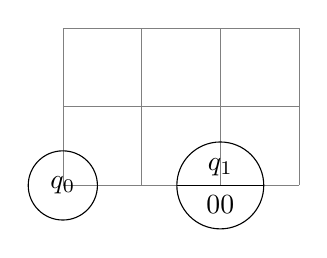
\begin{tikzpicture}
\draw[help lines] (0,0) grid (3,2);
\node[state without output] {$q_0$};
\node[state with output] at (2,0) {$q_1$ \nodepart{lower} $00$};
\end{tikzpicture}


\end{document}
